\documentclass[10pt,twocolumn,letterpaper]{article}

%%%%%%%%% PAPER TYPE  - PLEASE UPDATE FOR FINAL VERSION
% \usepackage[review]{cvpr}      % To produce the REVIEW version
\usepackage{cvpr}              % To produce the CAMERA-READY version
% \usepackage[pagenumbers]{cvpr} % To force page numbers, e.g. for an arXiv version

% Include other packages here, before hyperref.
\usepackage{graphicx}
\usepackage{amsmath}
\usepackage{amssymb}
\usepackage{booktabs}


% It is strongly recommended to use hyperref, especially for the review version.
% hyperref with option pagebackref eases the reviewers' job.
% Please disable hyperref *only* if you encounter grave issues, e.g. with the
% file validation for the camera-ready version.
%
% If you comment hyperref and then uncomment it, you should delete
% ReviewTempalte.aux before re-running LaTeX.
% (Or just hit 'q' on the first LaTeX run, let it finish, and you
%  should be clear).
\usepackage[pagebackref,breaklinks,colorlinks]{hyperref}


% Support for easy cross-referencing
\usepackage[capitalize]{cleveref}
\crefname{section}{Sec.}{Secs.}
\Crefname{section}{Section}{Sections}
\Crefname{table}{Table}{Tables}
\crefname{table}{Tab.}{Tabs.}


%%%%%%%%% PAPER ID  - PLEASE UPDATE
\def\cvprPaperID{*****} % *** Enter the CVPR Paper ID here
\def\confName{CVPR}
\def\confYear{2022}


\begin{document}

%%%%%%%%% TITLE - PLEASE UPDATE
\title{Compare Accuracy of Some ML Models on EEG Eye State Dataset}

\author{Afsaneh Shams\\
University of Georgia\\
{\tt\small as14847@uga.edu}
% For a paper whose authors are all at the same institution,
% omit the following lines up until the closing ``}''.
% Additional authors and addresses can be added with ``\and'',
% just like the second author.
% To save space, use either the email address or home page, not both
\and
Kushajveer Singh\\
University of Georgia\\
{\tt\small ks56866@uga.edu}
}
\maketitle
\graphicspath{ {./images/} }
%%%%%%%%% ABSTRACT
\begin{abstract}
   In this paper we discuss a framework for developing electroencephalography (EEG) based input methods. In particular, we focus on predicting the state of the eye of a person i.e. open or closed. This simple binary classification problem serves as the basis for a switching mechanism that all EEG based devices must support. In order to do this we first discuss our paradigm for collecting a dataset which can be extended to any other EEG based input method. And then to verify the effectiveness of the proposed binary binary classification problem we train several machine learning models including Random Forest, Decision Tree, Logistic Regression with the best model achieving 93.61\% accuracy on the given dataset, to show the effectiveness of this binary classification as a switching mechanism for various EEG based devices.
\end{abstract}

%%%%%%%%% BODY TEXT
\section{Introduction}
\label{sec:intro}

Human brain is a very complex structure with millions of neurons and with the development of electroencephalography (EEG), we can measure brain signals for various actions of a human body. To measure an EEG signal an EEG headset is used. In the recent years, the technology has advanced to the point where cheap EEG headsets offer the same advantages as the more expensive ones from a few years back, without compromising on the safety of the device. This has allowed a greater availability of these devices to the general public and with the increasing affordability of such devices it is paramount that we start looking into research directions which support EEG based input. This paper presents a general framework that can be used to add a easy switching mechanism in these EEG based input devices.

When developing technologies that rely on EEG based input, switching mechanisms are often required at various stages. These can include turning on/off a device, switching between different modes of operation. In the paper, we aim to provide a solution to this problem by transforming this problem to a binary classification problem. The binary classification problem can be based on any part of the human body, including moving a finger in a particular direction, moving the arm up or down, the state of the eye. The only constraint is that the desired activity should be able to be easily distinguished by the brain activity, without interference from other human activities.

As it is not possible to test every human motion that can be used for the switching mechanism, we focus on predicting the state of the eye of a person i.e. open or closed. We chose this particular human activity as an eye can be moved easily without moving the rest of the body which results in less interference in the brain activity from other parts of the body, making it a reliable method for various switching mechanisms. In the first part of the paper, we discuss the experimentation setup for collecting the data and then we discuss various machine learning models we used to solve the classification problem. 

We summarize our contributions as follows (1) discuss a general framework that can be used to collect the dataset for the switching problem (2) benchmark various machine learning models on the dataset to verify the effectiveness of the proposed method.

\section{Related Work}

Before EEG based signal, several papers focused on measuring the power of the signal when the eye is open or closed. \cite{paper1} was the first paper to observe that an eye state can be distinguished as open or closed based on the power of the signal. There are many limitations of this approach. The first limitation being power is only a single factor for classification and as a result the output can be easily altered if the input is corrupted. Also, it is difficult to isolate the power signal when predicting the state of the eye as the intensity can be easily influenced by various external factors that are not in control of the person. Follow up work by \cite{paper2} was the first paper to use artificial neural networks based on the EEG input signal. The authors of the above paper used very simple artificial neural networks to track the blinking of the eye, rather than to measure the state of the eye. Also, due to the simple algorithms used by the authors, the proposed method produced very poor performance.

\begin{figure*}
  \centering
  \begin{subfigure}{0.47\linewidth}
    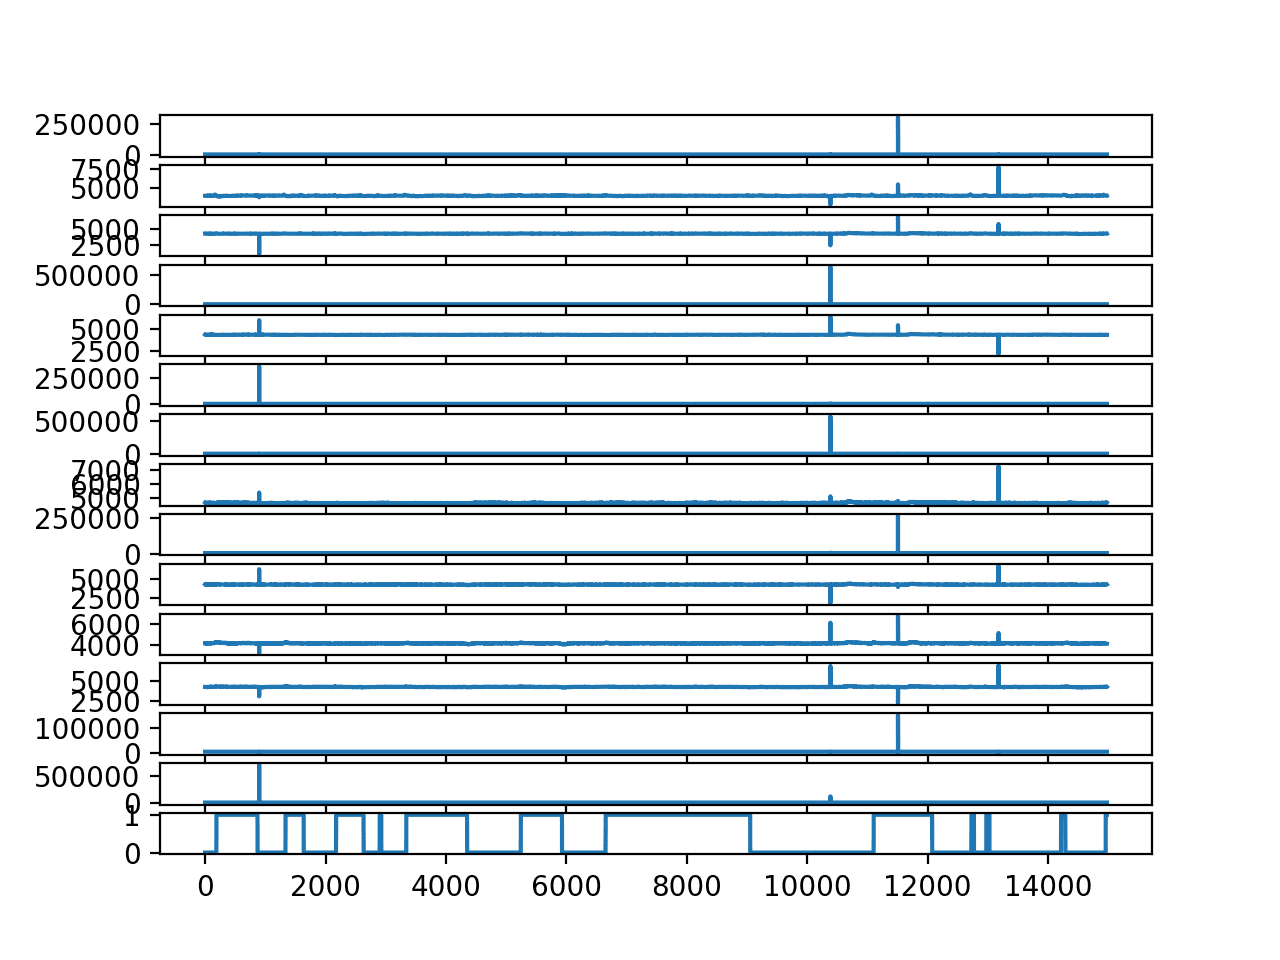
\includegraphics[width=\textwidth]{img1.png}
    % \fbox{\rule{0pt}{2in}
    % \rule{.9\linewidth}{0pt}}
    \caption{Line plot of input data with outliers.}
    \label{fig:short-a}
  \end{subfigure}
  \hfill
  \begin{subfigure}{0.47\linewidth}
    % \fbox{\rule{0pt}{2in} \rule{.9\linewidth}{0pt}}
    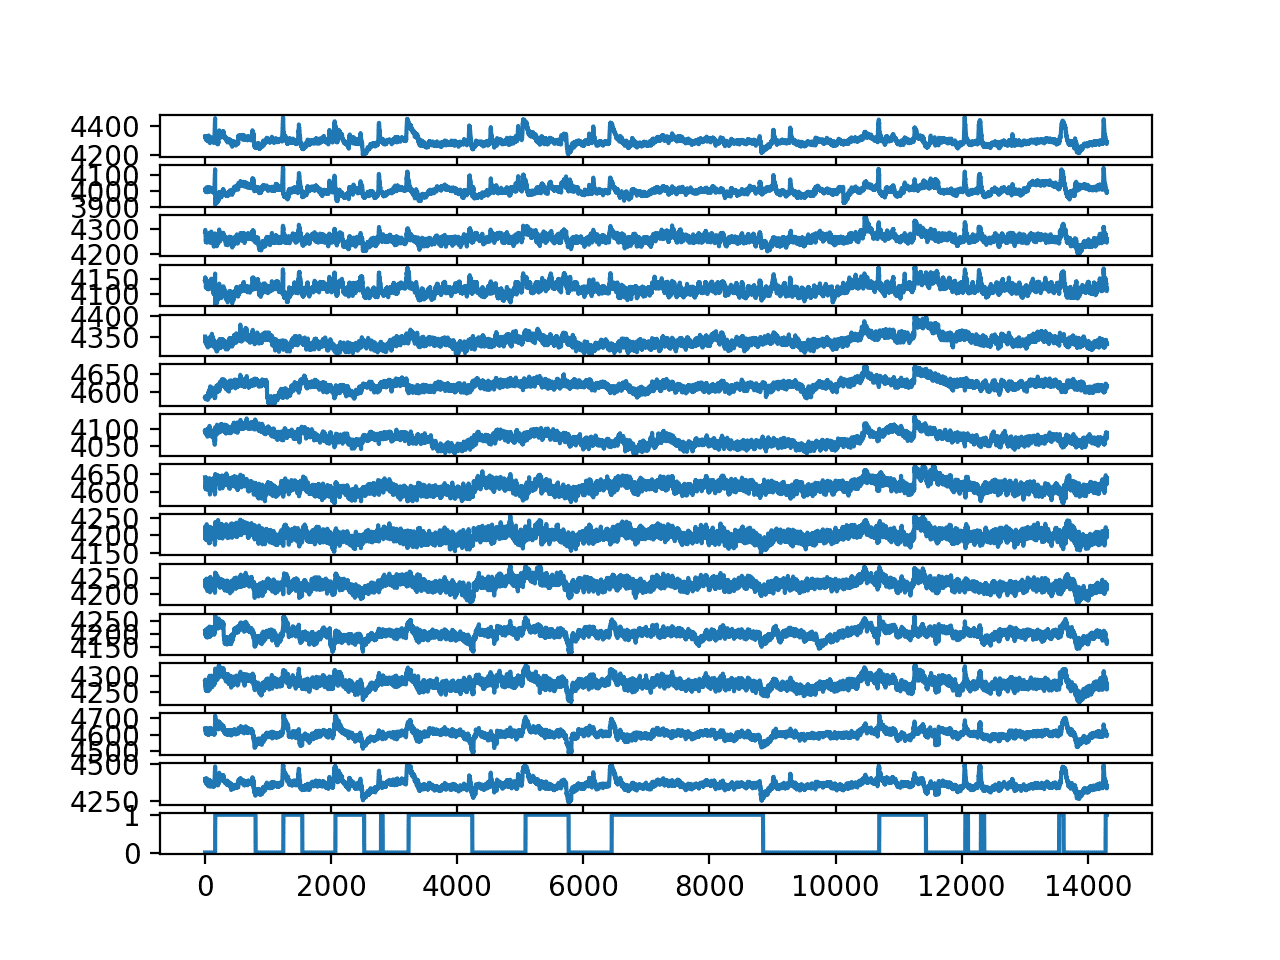
\includegraphics[width=\textwidth]{img2.png}
    \caption{Line plot of input data without outliers.}
    \label{fig:short-b}
  \end{subfigure}
  \caption{The input data is visualized using a line plot. In (a) the effects of outliers can be easily observed as there are many peaks which skew the data. In (b) all the data points that are four standard deviations away from the mean have been removed.}
  \label{fig:short}
\end{figure*}

\cite{paper3} also did a survey in which various algorithms and methods were proposed to tackle the problem for classification of the eye state. Although, the authors discussed the idea of using machine learning models to do classification but they never implemented an algorithm that can be used for the same. There is also an excellent review by \cite{paper4} on the topic that discuss the latest hardware and software used for EEG control signals.

In the next section we briefly discuss EEG headsets as these are the used to collect the data. An EEG headset consists of electrodes which are placed on the head. An EEG headset can have rigid electrodes that cannot be moved or flexible electrodes. Most of the consumer headsets have rigid electrodes. Another, factor is the sampling rate of the device i.e. the number of samples the device can record per second. Most consumer devices have a sampling rate of 256 samples a second. Another factor is the number of bits the device records for each sample. This controls how many voltage levels the device can measure.

\section{Data collection}

In this section, we describe the data collection system. The experiment begins by placing the person in a quite room without any distractions. The reason for doing this is we do not want the person's brain to spike when looking at these distractions as these can interfere with the results. Another important detail is to not tell the person when the experiment begins. This is essential to remove bias from the experiment. In the case of measuring the state of the eye of a person, if a person is told when the experiment begins then the person might subconsciously start thinking that they need to start blinking which can produce signals that have been interfered by this thinking. The person is just told to sit relaxed and look straight at the camera.

This experiment setup can be reproduced for any human activity that we wish to measure, like moving an arm or finger. The only constraints are the person is not told when the experiment begins and there are no unnecessary distractions.

\begin{table}
  \centering
  \begin{tabular}{@{}lc@{}lc@{}}
    \toprule
    Method & Accuracy \\
    \midrule
    Decision tree & 84.4993 \\
    Random Forest & \textbf{93.6115} \\
    Random Tree & 82.777 \\
    Naive Bayes & 46.769 \\
    Logistic Regression & 64.0988 \\
    Voted Perceptron & 55.1936 \\
    Bagging & 89.5327 \\
    \bottomrule
  \end{tabular}
  \caption{Results. All models were evaluated using 10-fold cross validation with the same random seed for the dataset splits. The reported accuracy is the average of all the runs. Random Forest achieved the highest accuracy and this accuracy is practical to implement a switching mechanism}
  \label{tab:example}
\end{table}

\section{Experiments}

We used an open-source dataset created by \cite{paper5}. The dataset consists of EEG signals as measured by the Emotiv EPOC headset. The task is to do binary classification to predict the state of the eye i.e. open or closed. The headset produces 15 features for each signal and the goal is to predict the state of the eye open (0) or closed (1) from these 15 features. These features represent the voltage levels as measured by the electrodes on the EEG headset. The dataset consists of 149,777 samples. To make the experiments fair, we did 10-fold cross validation for each model and then report the average.

The dataset contained no missing values but contained outliers. These outliers are probably due to some machine interference and we removed all the values that are four standard deviations from the mean. To remove the outliers all values outside the range of four standard devitations were removed. The effect of this is shown in Figure \ref{fig:short}.

To implement various machine learning algorithms we used the WEKA \footnote{http://old-www.cms.waikato.ac.nz/~ml/weka/} software. We tested several algorithms including decision trees, naive Bayes, logistic regression, voted perceptrons, bagging and random tree. The results are shown in Table \ref{tab:example}.

All the models were evaluated using 10-fold cross validation. The splits for cross validation were same for each model and to report the final accuracy we took the average of all the 10 runs. From the Table \ref{tab:example}. Standard classifiers like Naive Bayes, Logistic Regression, Voted perceptron performed very poorly as compared to to decision tree algorithms. Random forest was the best model we evaluated and the accuracy achieved by the model is practical and as a result, this model can be used to implement a switching mechanism in EEG based devices.

\section{Conclusion}

With the increasing affordability of EEG headsets, EEG based input methods are becoming increasing popular. In this paper, we presented a solution for the switching mechanism problem in these EEG devices. We selected the state of the eye as the human motion for doing the switching and using this we discussed a general data collection policy that can be used to measure any other human motion we want to use for switching. Various machine learning algorithms were also benchmarked to test the effectiveness of the proposed method and we found RandomForest to be the best model for solving this binary classification problem.

%%%%%%%%% REFERENCES
{\small
\bibliographystyle{ieee_fullname}
\bibliography{egbib}
}

\end{document}
